\documentclass[12pt,a4paper]{ctexart}

\usepackage[UTF8]{ctex}
\usepackage{geometry}
\usepackage{graphicx}
\usepackage{xcolor}
\usepackage{tikz}
\usepackage{fontspec}
\usepackage{setspace}
\usepackage{enumitem}
\usepackage{booktabs}
\usepackage{array}
\usepackage{longtable}
\usepackage{hyperref}
\usepackage{fancyhdr}
\usepackage{titlesec}
\usepackage{multicol}
\usepackage{xurl}
\usepackage{tocloft}

\renewcommand{\cfttoctitlefont}{\hfill\bfseries\Large}
\renewcommand{\cftaftertoctitle}{\hfill}
\geometry{left=2.5cm,right=2.5cm,top=2.5cm,bottom=2.5cm}

\definecolor{black}{RGB}{0,0,0}
\definecolor{mainblue}{RGB}{0,82,147}
\definecolor{accentgold}{RGB}{180,140,60}
\definecolor{lightgray}{RGB}{245,245,245}
\definecolor{darkgray}{RGB}{80,80,80}
\definecolor{mainred}{RGB}{230,1,45}

\hypersetup{
    colorlinks=true,
    linkcolor=black,
    urlcolor=mainblue,
    citecolor=mainblue,
    pdfborder={0 0 0}
}

\pagestyle{fancy}
\fancyhf{}
\fancyhead[L]{\small\color{darkgray}\textbf{量子行业每周新闻洞察}}
\fancyhead[R]{\small\color{darkgray}\textbf{总第192期}}
\fancyfoot[C]{\thepage}
\renewcommand{\headrulewidth}{0.4pt}
\renewcommand{\footrulewidth}{0pt}

\titleformat{\section}
    {\Large\bfseries\color{mainred}}
    {\thesection、}{0em}{}
\titleformat{\subsection}
    {\large\bfseries\color{mainred}}
    {\thesubsection、}{0em}{}

\newcolumntype{L}[1]{>{\raggedright\arraybackslash}p{#1}}
\newcolumntype{C}[1]{>{\centering\arraybackslash}p{#1}}

\begin{document}

% ==================== 封面 ====================
\begin{titlepage}
\begin{tikzpicture}[remember picture,overlay]
    \fill[mainred] ([yshift=-0.5cm]current page.north west) rectangle ([yshift=-1.2cm]current page.north east);
    \fill[mainred] ([yshift=1.2cm]current page.south west) rectangle ([yshift=0.5cm]current page.south east);
\end{tikzpicture}

\vspace*{4cm}

\begin{center}
    {\fontsize{44}{52}\selectfont\bfseries\color{black} \textbf{量子行业每周新闻洞察}}

    \vspace{0.8cm}

    {\fontsize{16}{22}\selectfont\color{darkgray} 2026.08.08 — 2026.08.14 }
    {\fontsize{16}{22}\selectfont\color{darkgray} \textbf{WEEKLY NEWS}}

    \vspace{1.5cm}

    {\fontsize{20}{26}\selectfont\color{mainred}\textbf{（总第\textbf{ 192 }期）}}

    \vspace{4cm}

    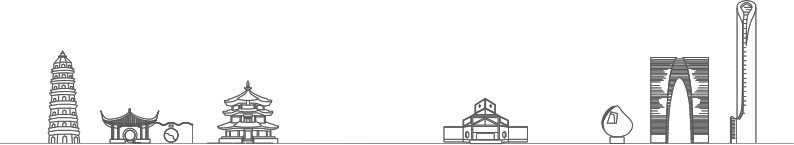
\includegraphics[width=\textwidth]{Cover_Suzhou.png}

    \vfill

    {\fontsize{12}{16}\selectfont\color{darkgray} 量子科技长三角产业创新中心\\编制：科技委办公室、产业发展部（理事会办公室）}
\end{center}
\end{titlepage}

% ==================== 目录 ====================
\pagenumbering{roman}
\newpage
\tableofcontents

\newpage

% ==================== 摘要 ====================
\pagenumbering{arabic}
\setcounter{page}{1}
\begin{center}
{\Large\bfseries\color{mainred} 摘\hspace{2em}要}
\end{center}
\addcontentsline{toc}{section}{摘要}


\textbf{ 宏观态势：}

本周该领域保持活跃态势。


\textbf{ 科技前沿：}

本周该领域保持活跃态势。


\textbf{ 产品动态：}

本周该领域保持活跃态势。


\textbf{ 企业资讯：}

本周该领域保持活跃态势。


\textbf{ 资本运作：}

本周该领域保持活跃态势。




\textbf{ 专利动态：}

本周专利动态涵盖低温环境系统、超导量子测控技术、量子软件与算法、量子算力网、量子科技长三角产业创新中心共5个板块、20条专利。




% ==================== 会议列表 ====================
{
    \newpage
    \section*{ 8月量子科技行业国内、国际会议}
    \addcontentsline{toc}{section}{ 8月量子科技行业国内、国际会议}
    \scriptsize
    \begin{longtable}{C{0.8cm}L{2.5cm}L{3cm}L{7cm}}
        \toprule[1.5pt]
        \textbf{序号} & \textbf{日期} & \textbf{地点} & \textbf{会议名称} \\
        \midrule
        \endfirsthead
        \toprule
        \textbf{序号} & \textbf{日期} & \textbf{地点} & \textbf{会议名称} \\
        \midrule
        \endhead
        \bottomrule
        \endfoot
        
        1 & 8月3日-5日 & 博尔德及线上, 美国 & 天气与气候应用的量子计算与传感研讨会 \\
        \midrule[0.05pt]
        
        2 & 8月3日-14日 & 贝纳斯克, 西班牙 & 容错量子技术研讨会 \\
        \midrule[0.05pt]
        
        3 & 8月7日-9日 & 杭州, 中国 & 第2届量子计算与通信技术国际会议（ICQCT 2026） \\
        \midrule[0.05pt]
        
        4 & 8月10日-14日 & 纳塔尔, 巴西 & 量子热力学会议2026（QTD 2026） \\
        \midrule[0.05pt]
        
        5 & 8月10日-14日 & 阿姆斯特丹, 荷兰 & QSim2026 \\
        \midrule[0.05pt]
        
        6 & 8月14日-16日 & 印第安纳波利斯, 美国 & 量子AI与自然语言处理2026会议（QNLPAI 2026） \\
        \midrule[0.05pt]
        
        7 & 8月16日-21日 & 巴德洪内夫, 德国 & 量子机器学习暑期学校（Bad Honnef物理学校） \\
        \midrule[0.05pt]
        
        8 & 8月16日-22日 & 贝纳斯克, 西班牙 & 悬浮系统量子工程研讨会 \\
        \midrule[0.05pt]
        
        9 & 8月17日-21日 & 多伦多, 加拿大 & 第11届量子信息与量子控制会议（CQIQC-XI） \\
        \midrule[0.05pt]
        
        10 & 8月17日-21日 & 阿姆斯特丹, 荷兰 & 第23届量子物理与逻辑国际会议（QPL 2026） \\
        \midrule[0.05pt]
        
        11 & 8月24日-28日 & 渥太华, 加拿大 & QCrypt 2026 \\
        \midrule[0.05pt]
        
        12 & 8月24日-28日 & 大田, 韩国 & 第26届亚洲量子信息科学会议 (AQIS) \\
        \midrule[0.05pt]
        
        13 & 8月24日-28日 & 维也纳, 奥地利 & 第9届青年量子信息科学家国际会议 (YQIS) \\
        \midrule[0.05pt]
        
        14 & 8月25日-28日 & 哥德堡, 瑞典 & 超导量子比特与算法 2026 (SQA) \\
        \midrule[0.05pt]
        
        15 & 8月30日-9月1日 & 布雷钦, 英国 & 量子ARC写作静修 \\
        \midrule[0.05pt]
        
        16 & 8月31日-9月3日 & 仁川, 韩国 & 硅量子电子学研讨会 2026 (SiQEW) \\
        \midrule[0.05pt]
        
        17 & 8月31日-9月3日 & 泰恩河畔纽卡斯尔, 英国 & Photon 2026 \\
        \midrule[0.05pt]
        
        18 & 8月31日-9月4日 & 瓦莱塔, 马耳他 & Qalypso 2026暑期学校—量子优化技术与计算物理 \\
        \midrule[0.05pt]
        
        19 & 8月31日-9月4日 & 舍布鲁克, 加拿大 & 量子计算、通信与密码学理论 2026 (TQC) \\
        \midrule[0.05pt]
        
        20 & 8月31日-9月10日 & 格但斯克, 波兰 & Q-Camp: 量子暑期学校 2026 \\
        \midrule[0.05pt]
        
    \end{longtable}
}




% ==================== 宏观态势 ====================
\newpage
\section{宏观态势}
\vspace{-0.5em}
\noindent\rule{\linewidth}{1.5pt}

\subsection{ D-Wave获加拿大国家研究委员会资助，将推进退火量子计算软件研发 }

2026年08月14日消息，量子计算公司D-Wave日前宣布，它已获得加拿大国家研究委员会（NRC）应用量子计算挑战项目提供的30万加元资助，将推进退火量子计算商用软件研发。D-Wave位于不列颠哥伦比亚省本拿比的量子工程卓越中心团队将与NRC合作，开发下一代软件和算法，帮助企业在Advantage2退火量子计算机上解决更大、更复杂的优化问题。该项目将针对Zephyr拓扑创建新的图子式嵌入算法，并将其集成至公司开源Ocean软件开发套件中。该算法是优化问题映射到Advantage2系统拓扑的基础过程，有望扩大Advantage2系统可处理的计算规模和复杂度。

\noindent\textbf{报道链接：}\url{https://www.dwavequantum.com/company/newsroom/press-release/d-wave-awarded-national-research-council-of-canada-funding/}

\subsection{ 美国犹他州签署行政令，量子技术升级为该州未来经济战略重点 }

2026年08月13日消息，美国犹他州州长近日签署一份行政命令，正式发布“犹他量子倡议”，将量子技术列为该州经济战略重点，以加速相关研究、商业化、劳动力开发和先进制造。根据行政命令，犹他州州长经济发展办公室将牵头组建量子协调委员会，汇集州政府、高等教育和产业界代表，统筹犹他州量子战略，以提升该州对私人投资和联邦项目的吸引力。犹他州州长表示，量子技术将改变计算、通信、制造、药物研发和国防方式，犹他州已拥有世界级研究力量、半导体与先进制造基础以及国防资产，该倡议旨在串联这些优势，培养面向未来的劳动力体系，确保未来技术能在该州完成发明、制造与应用落地。

\noindent\textbf{报道链接：}\url{https://thequantuminsider.com/2026/08/10/utah-launches-quantum-initiative/}

\subsection{ 美国国防部启动Farseer项目 推动量子传感器与时钟融入ISR系统 }

2026年08月11日消息，美国国防部下属国防创新部门（DIU）已于7月启动一项名为Farseer的多阶段项目，旨在将成熟的量子传感器与时钟技术快速转化，集成至情报、监视与侦察（ISR）系统的精确授时、定位与导航（A-PNT）能力中。据悉，该项目将重点利用量子传感技术，在维持ISR任务要求的同时突破传统尺寸、重量与功耗（SWaP）限制。其招标文件指出，量子传感器和时钟不受经典系统底层局限的约束，可同时实现高灵敏度与低SWaP。

\noindent\textbf{报道链接：}\url{https://www.janes.com/defence-intelligence-insights/defence-news/defence/pentagon-launches-farseer-quantum-sensing-initiative}


% ==================== 科技前沿 ====================
\newpage
\section{科技前沿}
\vspace{-0.5em}
\noindent\rule{\linewidth}{1.5pt}

\subsection{ A*STAR量子创新中心开发出超低损耗悬浮转子，可用于推进精密传感和探索量子行为 }

2026年08月14日消息，新加坡科技研究局量子创新中心（A*STAR）的研究团队开发出一种毫米级悬浮转子，在驱动关闭后持续旋转了超过10小时，实现了该尺寸机械转子迄今最低的能量耗散率。团队通过实时控制和精确施加静电力，将转子加速至每分钟930转，并在高真空环境下维持长时间运行。该平台可检测低至每秒0.0065度的旋转速率，灵敏度已达到商业级陀螺仪水平。研究人员称，这种具有低能量损失的大型转子建立了一个平台，可用于推进精密传感和探索大型机械系统中的量子行为。

\noindent\textbf{报道链接：}\url{https://www.eurekalert.org/news-releases/1139787}

\subsection{ 帝国理工学院研究人员合作提出新型光子量子计算架构Clavina }

2026年08月13日消息，英国帝国理工学院物理系联合外部合作者近日在《自然·光子学》发表一项研究成果，提出一种名为Clavina的新型可编程量子计算架构，它可在单一系统中同时实现线性与非线性量子操作，克服了光子量子计算长期存在的功能限制。研究团队利用该系统模拟了凝聚态物理中描述量子粒子相互作用的玻色-哈伯德模型，并进一步演示了一种更可靠的GKP态生成方法——GKP态被认为是量子纠错的重要资源。该进展有望拓展基于光的量子计算机在量子模拟与容错计算方面的能力。

\noindent\textbf{报道链接：}\url{https://phys.org/news/2026-08-shifting-architecture-versatility-photonic-quantum.html}

\subsection{ 我国科学家通过理论建模预测：双层硼烯材料可在常压下实现68K超导临界温度 }

2026年08月13日消息，我国科学家通过理论建模预测，堆叠两层微观硼层可刷新超导临界温度新纪录。目前已知性能最佳的元素超导体钪，需在约260 GPa压力下才能达到36K（-237°C）的临界温度；而新研究预测，采用AA堆叠结构的双层硼烯在常压下即可实现68K（-205°C）的超导临界温度。与传统二维材料依靠弱相互作用不同，双层硼烯层间由强共价硼-硼键连接，这一结构改变了原子振动方式，为在更高温度下实现超导开辟了新途径。由于该结果完全基于理论计算，研究团队表示，实验验证将是他们下一步工作的重要方向。

\noindent\textbf{报道链接：}\url{https://phys.org/news/2026-08-boron-layers-superconductivity-theoretical.html}

\subsection{ Pasqal旗下子公司成功实现在光子芯片上激光捕获单个原子 }

2026年08月12日消息，中性原子量子计算企业Pasqal日前宣布，其于18个月前收购的子公司Aeponyx，在全球首次利用光子集成电路（PIC）产生的激光捕获了单个原子。Pasqal称，该突破标志着可扩展的量子比特控制方法取得新进展，有望支撑未来大规模容错量子计算处理器。在该演示中，Pasqal通过单个光子芯片生成四个光镊，并用它们将四个单独的铷原子固定在量子处理单元内。测试表明，该光子芯片架构的原子捕获性能与现有bulk光学系统相当，原子寿命约为27.5秒。该平台结合了Aeponyx的氮化硅光子学技术，旨在将未来处理器的光学占用空间缩小至多50倍，并为大规模制造开辟实用路径。

\noindent\textbf{报道链接：}\url{https://www.pasqal.com/newsroom/pasqal-brings-qubit-control-on-chip-advancing-the-path-to-fault-tolerant-quantum-computing-at-scale/}

\subsection{ Quemix获本田投资，加速量子算法与软件技术走向实际应用 }

2026年08月12日消息，日本量子算法与软件研发企业Quemix近日宣布，它已获得本田技研工业株式会社的投资。Quemix与本田此前通过量子计算联合研究取得了一系列开创性成果：2025年5月，双方合作开发出全球首创的量子态读取新技术；同年6月，双方研发出一种可在量子计算机上对密度泛函理论（DFT）计算实现指数级加速的新量子算法。Quemix表示，此次投资将加速其提升产品与服务价值，推动量子计算走向实际应用。

\noindent\textbf{报道链接：}\url{https://www.quemix.com/en/post/en-20260807-honda}

\subsection{ Quantum Optics Jena公司的量子通信系统通过六项独立安全测试 }

2026年08月11日消息，Quantum Optics Jena近日宣布，其ELVIS量子通信系统已通过由TÜV Informationstechnik执行的六项独立安全测试，测试依据ISO/IEC 23837标准开展。此次评估聚焦于量子密钥分发（QKD）系统中激光器、探测器及光学元件等组件可能遭受的硬件侧信道攻击。该公司表示，此次测试结果将有助于推动商业量子通信系统安全认证标准的制定。

\noindent\textbf{报道链接：}\url{https://thequantuminsider.com/2026/08/06/quantum-optics-jena-unhackable-quantum-communication-independent-security-test/}

\subsection{ 加州理工学院利用纠缠光子对实现四倍量子增强的显微镜分辨率 }

2026年08月11日消息，三年前，加州理工学院科学家团队证明纠缠光子对可使光学显微镜分辨率翻倍。如今，该团队采用新光学设计，将其中一个纠缠光子三次通过显微镜光学系统，实现了比经典显微镜约四倍的分辨率提升。团队利用标准测试目标对比经典成像、此前的二倍量子配置及新的三通道配置，结果表明，二倍配置相比经典成像分辨率提高约1.8倍，新配置则实现约4倍增强。该技术有望用于半导体器件检测，在需要长波长但经典光学分辨率受限的场景下，四倍分辨率提升可显著增强芯片缺陷的识别能力。

\noindent\textbf{报道链接：}\url{https://phys.org/news/2026-08-quantum-microscopy-quadruples-microscope-resolution.html}

\subsection{ 磁性掺杂量子点可用于捕获热电子，有望加速驱动光化学反应 }

2026年08月10日消息，美国洛斯阿拉莫斯国家实验室科学家近日在《自然通讯》发表的研究中，展示了一种可显著拓展光驱动化学应用范围的新型量子点机制。通过在半导体量子点中引入磁性锰掺杂剂，团队构建出一条超快自旋交换路径，能够在热电子能量以热量形式耗散前将其捕获，并用于驱动化学还原反应。该研究以甲基紫精作为模型分子受体，直接证明了磁性掺杂剂可实现量子点中的高效热电子还原。实验显示，锰掺杂量子点的电子转移速度显著快于未掺杂颗粒，即使常规带边能量条件不利，仍能驱动还原反应。

\noindent\textbf{报道链接：}\url{https://phys.org/news/2026-08-magnetic-dopants-quantum-dots-chemical.html}

\subsection{ 莱斯大学科学家开发出能精确调节离子阱模拟器内部温度的新方法 }

2026年08月10日消息，莱斯大学研究团队开发出一种能精确调节离子阱模拟器内部温度的新方法，使量子模拟能在更贴近真实条件的设定温度下运行，成果已发表于《物理评论快报》。团队设计了一个“双旋钮”控制系统，将加热和冷却独立调节：一方面以精密激光束持续清除离子运动的振动能量产生冷却，另一方面利用腔室外天线发射射频信号随机扰动离子产生加热。通过平衡两者强度，可精确设定模拟器温度。在首次测试中，团队模拟了化学反应中电子在分子间转移的电荷转移过程；第二次测试则模拟了受植物光合作用启发的能量传输，发现精确加热可解锁隐藏能量通道，使能量跨越在低温下无法逾越的障碍。该成果有助于离子阱量子模拟器更真实地模拟化学与生物过程。

\noindent\textbf{报道链接：}\url{https://phys.org/news/2026-08-temperature-dial-realistic-quantum-simulations.html}

\subsection{ 美研究团队在原子薄半导体中观察到可调谐激子玻色-爱因斯坦凝聚 }

2026年08月10日消息，由劳伦斯伯克利国家实验室领导的研究团队近日在《自然》杂志发表一项成果，他们在原子级厚度的半导体中，于高温条件下观察到可调谐的激子玻色-爱因斯坦凝聚（BEC）。该研究发现，这些激子不仅形成了凝聚体，其内部结构还可通过磁场进行切换。实验中，团队采用低温磁光光谱技术，将器件冷却至接近绝对零度，并借助电学栅极调控激子密度，以测量电子和空穴组分对微弱磁场的响应。令人意外的是，凝聚态特征在约2开尔文的温度下依然存在——尽管仍极冷，但已比此前超冷原子气体中的BEC演示温度高出数百万倍。

\noindent\textbf{报道链接：}\url{https://physics.berkeley.edu/news/scientists-reveal-hidden-structure-quantum-fluid}

\subsection{ 德国哥廷根大学研究团队成功成像纳米有机分子三维波函数 }

2026年08月10日消息，德国哥廷根大学的一个跨学科研究团队成功对一个纳米尺度有机分子的三维波函数进行了成像。团队将最先进的光电子能谱技术与强大的数学算法相结合，克服了此前观测方法的限制。该方法引入了两个新概念：一是从底层重新设计计算机算法，使可靠的三维图像得以用更少的实验数据获得；二是采用基于实验室的软X射线光源，提供超短光脉冲。正是这两项技术的结合产生了显著效果，现在只需使用远少于以往的实验数据，就能获得可靠的3D图像。

\noindent\textbf{报道链接：}\url{https://www.uni-goettingen.de/en/3240.html?id=8252}

\subsection{ 日本科学家利用量子涨落理论框架揭示手性磁体异常导电行为 }

2026年08月10日消息，东京科学大学的研究人员近期在《物理评论快报》上发表一篇论文，提出了一套基于量子涨落的理论框架，用于解释手性磁体中方向依赖的电流输运现象。在手性磁系统中，电流的导电行为会随流动方向而改变，但量子效应在此过程中的作用此前尚不明确。该团队发现，手性磁体中的非互易电流与金属中一种已知的量子现象之间存在出乎意料的关联。这一发现有望为自旋电子学的发展提供关键理论支撑。

\noindent\textbf{报道链接：}\url{https://educ.titech.ac.jp/phys/eng/news/2026\_08/069974.html}

\subsection{ 波士顿学院团队开发出可捕获带电激子的电可调量子纳米围栏 }

2026年08月10日消息，美国波士顿学院的物理学家门近日在《自然·纳米技术》发表一项成果，制造出一种电可调量子纳米围栏，可捕获带电激子，并对微小光源的亮度、颜色和量子态进行精确电控。团队在单层二硒化钨二维半导体中研究了复合带电激子，利用纳米多孔金属单层材料钽铱碲化物作为电场掩膜，构建了静电“纳米围栏”，产生微小且聚焦的电场，使带电粒子受周围中性粒子束缚而固定在原位。这一成果为量子光源的精确操控提供了新方法。

\noindent\textbf{报道链接：}\url{https://www.eurekalert.org/news-releases/1138929}

\subsection{ 研究人员在微重力条件制备出铷钾原子BEC混合物，实现前所未有原子通量 }

2026年08月10日消息，一个国际研究团队在《自然通讯》上报告称，他们利用德国汉诺威莱布尼茨大学爱因斯坦电梯中的MAIUS-B装置，在微重力条件下制备并研究了由铷和钾两种原子构成的玻色-爱因斯坦凝聚体（BEC）混合物，实现了前所未有的原子通量。该系统的关键组成部分——位于激光模块与真空系统之间的光学平台，由美因茨约翰内斯·古腾堡大学和汉堡大学联合开发。光学平台采用微晶玻璃材料Zerodur制成，其极低的热膨胀系数确保能在火箭发射的极端机械载荷和温度变化下仍能精确控制原子。

\noindent\textbf{报道链接：}\url{https://press.uni-mainz.de/high-precision-laser-system-enables-record-flux-of-quantum-gas-mixtures/}

\subsection{ 新研究利用阳光直接产生纠缠光子，有望为卫星量子加密开辟可能 }

2026年08月10日消息，在发表于《Optica》的一项新研究中，加拿大渥太华大学与德国马克斯·普朗克光科学研究所（MPL）合作，利用新型锥形太阳能聚光器，从天然阳光中直接产生了纠缠光子。这一进展结合了渥太华大学团队的理论研究与MPL团队开发的新型太阳能聚光装置。实验结果显示，在考虑输入光带宽差异后，阳光源的纠缠质量可与激光源方案相媲美。通过量子态层析测量，所得纠缠态与理想纠缠态的相似度约为94\%；光子关联测量违反贝尔不等式，证实其关联源于量子纠缠而非经典效应。该技术未来有望使卫星利用太空中充足的阳光直接生成安全加密密钥，降低对地面激光器的依赖。

\noindent\textbf{报道链接：}\url{https://www.eurekalert.org/news-releases/1138247}

\subsection{ 亚马逊AWS密码学家提出针对二面体陪集问题的多项式时间量子算法 }

2026年08月10日消息，亚马逊AWS密码学组的科学家近日发布一篇预印本论文，提出一种针对二面体陪集问题的多项式时间量子算法。该算法据称消除了此前方法的关键限制，并可容忍部分有缺陷的量子样本。若该结果通过独立验证，将强化量子计算机可高效求解格问题的理论依据，而这类问题正是当前大量后量子密码的安全基础。不过，该论文并未展示对标准化后量子密码的实际攻击，也未估算所需量子硬件资源。后续独立分析需验证其“擦除方法”在假设条件下是否成立、递归过程中概率界是否保持，以及转换为显式量子电路后的复杂度表现。

\noindent\textbf{报道链接：}\url{https://thequantuminsider.com/2026/08/06/amazon-researcher-claims-quantum-algorithm-could-challenge-pqc-foundations/}


% ==================== 产品动态 ====================
\newpage
\section{产品动态}
\vspace{-0.5em}
\noindent\rule{\linewidth}{1.5pt}

\subsection{ 韩国延世大学将升级其IBM量子计算机至Nighthawk量子处理器 }

2026年08月14日消息，韩国延世大学通过其量子计划宣布，将于11月把其IBM量子计算机的量子处理单元（QPU）升级为Nighthawk量子处理器。目前全球唯一一个部署有Nighthawk量子计算机的站点是IBM迈阿密数据中心，延世大学有望成为全球第二个拥有基于该处理器的量子计算机的研究机构。同期，该计划将推出“Q-Bridge”平台，以支持工业界使用量子计算。

\noindent\textbf{报道链接：}\url{https://en.sedaily.com/technology/2026/08/12/yonsei-to-build-worlds-second-nighthawk-quantum-computer?utm\_source=chatgpt.com}

\subsection{ Quantinuum与甲骨文达成战略合作 将把量子计算引入至后者云基础设施平台 }

2026年08月14日消息，量子计算公司Quantinuum与甲骨文（Oracle）日前共同宣布达成一项为期多年的战略合作，计划将量子计算引入Oracle云基础设施（OCI）。根据合作协议，OCI用户将能够通过该平台的量子服务，直接访问Quantinuum的Helios量子计算系统，同时还能使用OCI的HPC和GPU基础设施。甲骨文计划在未来几个月提供其OCI量子服务的预览版本，从而为开发人员提供一种从量子计算模拟过渡到在真实量子计算硬件上执行应用的简化方法。

\noindent\textbf{报道链接：}\url{https://www.quantinuum.com/press-releases/quantinuum-and-oracle-partner-to-accelerate-hybrid-quantum-compute-adoption-on-oracle-cloud-infrastructure}

\subsection{ 韩国SDT加入Open Quantum Design，将参与开源量子处理器设计与开发 }

2026年08月14日消息，韩国量子计算企业SDT Inc.最近加入了加拿大非营利组织Open Quantum Design（OQD）。SDT专注于全栈量子计算机的设计和制造，此次加入OQD后将与全球成员机构共同参与开源量子处理器的设计与开发，并推动相关技术在亚洲地区的应用。据了解，OQD是一个致力于降低量子硬件研发门槛的开放平台，成员包括多家大学、实验室及企业，它通过共享设计和工具，来加速量子计算技术的迭代。

\noindent\textbf{报道链接：}\url{https://openquantumdesign.org/founders-\%26-physicists/f/koreas-sdt-quantum-joins-open-quantum-design}

\subsection{ Aquark与英国皇家海军等伙伴完成首次量子定时雷达网络试验 }

2026年08月13日消息，量子技术公司Aquark Technologies最近联合英国皇家海军、Saab UK、Qinetiq及英国国防科学技术实验室（DSTL），成功完成一项试验，它利用皇家海军舰艇雷达系统提供精确导航信息。试验于2026年6月进行，使用了Saab与Qinetiq场地的雷达，皇家海军实验船与DSTL作为网络转发节点。试验中，两台基于量子的时间服务器被部署至两个地理位置分离的站点，从冷启动至输出合格定时信号用时不到30分钟。且两个雷达系统仅依靠AQlock的计时来创建单一、准确的空中图像，并模仿了典型的GNSS拒绝和GNSS欺骗条件。

\noindent\textbf{报道链接：}\url{https://www.aquarktechnologies.com/post/aquark-augments-networked-radars-with-quantum-based-timing-in-first-of-its-kind-trial}

\subsection{ Qunnect与Monarch Quantum达成战略合作，加速可部署量子网络基础设施商业化 }

2026年08月12日消息，量子网络基础设施开发商Qunnect与量子光子学公司Monarch Quantum于日前宣布建立战略合作伙伴关系，以加速可部署量子网络基础设施的商业化进程。双方将结合Qunnect经现场验证的量子网络技术与Monarch Quantum在光子系统工程、产品化、小型化及可扩展制造方面的专长，共同开发模块化、可制造的量子网络硬件，并面向商业、工业、国防、太空及关键基础设施等应用场景。该合作将基于Qunnect于2024年推出的交钥匙型商用纠缠分发系统Carina，开发更紧凑、更易部署的衍生型号，以满足对尺寸、重量、功耗和操作灵活性要求较高的量子网络安装环境。

\noindent\textbf{报道链接：}\url{https://monarchquantum.com/2026/08/09/qunnect-and-monarch-quantum-partner-to-commercialize-deployable-quantum-networking-infrastructure/}

\subsection{ QC Ware利用IBM量子硬件完成混合量子-经典化学工作流演示 }

2026年08月11日消息，近日，美国量子软件公司QC Ware宣布，它利用其Promethium平台与IBM Quantum硬件完成了一项混合量子-经典计算化学工作流技术演示。该演示结合GPU加速分子建模与经典化学方法，在IBM 156比特Heron超导量子处理器上执行量子测量，成功计算出氧化亚氮还原酶的静电相互作用能，展示了Promethium在科学相关流程中对接量子硬件的可行性。不过QC Ware表示，此项演示属于技术验证，尚未成为Promethium产品的完整集成功能。

\noindent\textbf{报道链接：}\url{https://www.hpcwire.com/off-the-wire/qc-ware-demonstrates-hybrid-quantum-classical-chemistry-workflow-with-ibm-quantum/}

\subsection{ 德国研究团队开发可扩展量子光子芯片架构，6×6单光子源阵列工作良率达100\% }

2026年08月10日消息，德国柏林工业大学联合奥尔登堡大学的研究人员近日在《光：科学与应用》上发表一项研究，他们提出一种可扩展的量子光子芯片架构。该架构将确定性定位的半导体量子发射器集成至纳米光子谐振器，无标记集成策略省去了耗时定位与对准流程，突破了传统扩展瓶颈。团队制备了6×6器件阵列，工作良率达100\%。其中性能最佳器件的光子提取效率接近50\%，单光子纯度超过99\%，同时保持了窄光学线宽和高不可区分性，能满足先进光子量子处理器的关键需求。该技术兼容现有半导体制造工艺，为晶圆级量子光子硬件提供了现实路径，有望加速安全量子通信、紧凑型量子传感及大规模确定性单光子源光学量子计算架构的发展。

\noindent\textbf{报道链接：}\url{https://www.eurekalert.org/news-releases/1138966}



% ==================== 专利动态 ====================
\newpage
\section{专利动态}
\vspace{-0.5em}
\noindent\rule{\linewidth}{1.5pt}

\subsection{ 低温环境系统 }

\subsubsection{ 一种基于浮栅晶体管量子隧穿效应的真随机数生成方法及装置 }

申请人：陈立波

发明人：陈立波

公开日/授权日：2026-08-11

摘要：

本申请公开了一种基于浮栅晶体管量子隧穿效应的真随机数生成方法及装置。该方法包括：利用至少一个浮栅晶体管作为熵源，所述浮栅晶体管的栅氧化层厚度不小于20纳米，其栅极漏电流由量子隧穿效应主导；采集所述浮栅晶体管的栅极漏电流量子涨落信号；对所述量子涨落信号进行密码哈希后处理，输出真随机数；上述全部步骤均由纯硬件电路执行，无任何软件处理器参与。本申请能够在宽温度范围内提供稳定的真随机数输出，解决了现有技术在低温环境下随机性不足的问题，提高了电子设备的安全性和可靠性。

\noindent\textbf{专利链接：}\url{https://analytics.zhihuiya.com/patent-view/abst?patentId=cf9e0720-59ab-4a22-98a5-a4c9c0529608&shareId=68323BF7-F867-5E5B-3C1B-906779E4B656&from=EXPORT&signature=ioJm4%2BbLBvveLyS%2FLs705dwMO0CS%2FA3eVt%2BmOFy%2BALs%3D&expire=94608000&date=20260814T005524Z&version=1.0}

\subsubsection{ 一种基于超导磁悬浮稳控的金刚石NV色心量子纠缠远程通信系统 }

申请人：郭大干

发明人：郭大干

公开日/授权日：2026-08-11

摘要：

本发明公开一种基于超导磁悬浮稳控的金刚石Nv色心量子纠缠远程通信系统，包含近端与远端对称双向通信终端，终端内置编码与读取物理隔离的金刚石NV色心量子阵列，近端编码区(Al区)、读取区(B1区)分别与远端编码区(A2区)、读取区(B2区)一一对应，配对形成量子纠缠对。本发明采用非自由空间分发模式，不发射量子比特、不通过光纤传输量子态，纠缠制备与读取均在封闭局域体系内完成。系统采用复合超高真空腔体、钼合金电磁屏蔽、4.2K超导磁悬浮稳控，可移动异地部署，通过局域磁场编码(编码区自旋向上对应“1”、向下对应“0”)与磁信号读取，实现无延迟、无电磁发射的安全通信。

\noindent\textbf{专利链接：}\url{https://analytics.zhihuiya.com/patent-view/abst?patentId=0e6cbb17-4125-43b3-9b7d-2029185e0c49&shareId=68323BF7-F867-5E5B-3C1B-906779E4B656&from=EXPORT&signature=9JJL2qrhfuv1v4nXTgxo2Pzuqem9ES3yU9baAvCkmeg%3D&expire=94608000&date=20260814T005524Z&version=1.0}

\subsubsection{ 利用基带脉冲实现量子比特的可扩展控制 }

申请人：麻省理工学院

发明人：OLIVER, WILLIAM D. | GUSTAVSSON, SIMON

公开日/授权日：2026-08-11

摘要：

根据本发明的一个方面,一种用于执行量子计算的系统包括:第一环境,用于维持在环境温度下,具有经典计算处理器;以及第二环境,用于维持在低温温度下,具有多个量子比特和耦合到所述多个量子比特的多路复用电路,所述多个量子比特中的每一个都具有能隙跃迁频率;其中,所述经典计算处理器被配置为通过控制所述多路复用电路将所述多个量子比特中的特定一个耦合到脉冲基带波形来改变所述多个量子比特中每一个的状态。

\noindent\textbf{专利链接：}\url{https://analytics.zhihuiya.com/patent-view/abst?patentId=8fa59217-49df-4aa5-b153-1b98e1944f71&shareId=68323BF7-F867-5E5B-3C1B-906779E4B656&from=EXPORT&signature=YgzPy8pmxcFFyGRy6Z9FwSgeBk1mgWcemOzKHk2VP5U%3D&expire=94608000&date=20260814T005524Z&version=1.0}

\subsubsection{ 模块化量子资源态系统 }

申请人：匹西量子公司

发明人：GIMENO-SEGOVIA, MERCEDES | SPARROW, CHRISTOPHER | VOROBEICHIK, ILYA

公开日/授权日：2026-08-11

摘要：

模块化量子纠缠处理系统可以包括多个种子态系统、资源态系统和融合系统,这些系统可以以不同的方式排列。这些系统可以由模块化组件或芯片组成,从而实现模块化和扩展,以可扩展的方式执行基于纠缠的任务处理。不同系统中的某些组件或芯片可以设计为在低温下运行,例如探测器;而其他组件或芯片则可以在室温下运行,不同类型的芯片可以通过光纤电缆相互耦合。

\noindent\textbf{专利链接：}\url{https://analytics.zhihuiya.com/patent-view/abst?patentId=0d00b83e-c265-494e-8808-1e1ba7d67e10&shareId=68323BF7-F867-5E5B-3C1B-906779E4B656&from=EXPORT&signature=rZg4yGgP6%2FxnSlrEW3T%2FkO6EhqaKj2rtEJ%2Fsyp6bT%2BE%3D&expire=94608000&date=20260814T005524Z&version=1.0}

\subsubsection{ 高电子迁移率晶体管,其栅极电极位于沟道下方 }

申请人：国际商业机器公司

发明人：ZOTA, CEZAR BOGDAN | CHA, EUNJUNG | MORF, THOMAS | MUELLER, PETER

公开日/授权日：2026-08-11

摘要：

本文提供的一种或多种系统、装置、使用方法和/或制造方法涉及一种栅极位于沟道下方的高电子迁移率晶体管。根据一个实施例,该装置包括源极和漏极,它们耦合到高电子迁移率晶体管(HEMT)异质结构的顶面,以及栅极,该栅极与HEMT异质结构的底面接触。

\noindent\textbf{专利链接：}\url{https://analytics.zhihuiya.com/patent-view/abst?patentId=992394cf-ea56-4345-8926-af9114d15a3e&shareId=68323BF7-F867-5E5B-3C1B-906779E4B656&from=EXPORT&signature=WnuyV3UumowAlCsvT3c024bPBiVRbv8LKWEctmARNtM%3D&expire=94608000&date=20260814T005524Z&version=1.0}


\subsection{ 超导量子测控技术 }

\subsubsection{ 量子计算系统的全局控制 }

申请人：迪拉克私人有限公司

发明人：A·祖拉克 | J·J·普拉

公开日/授权日：2026-08-11

摘要：

公开了用于控制量子处理器中的一个或多个量子位的系统和方法。所述系统包括具有一个或多个基于自旋的量子位的量子处理器以及定位于量子处理器附近的介电谐振器。介电谐振器提供磁场。量子处理器定位于由谐振器提供的磁场的一部分中，使得磁场的一部分控制量子处理器的一个或多个基于自旋的量子位的自旋跃迁。

\noindent\textbf{专利链接：}\url{https://analytics.zhihuiya.com/patent-view/abst?patentId=442ac94e-c2b3-4601-89ca-89a9d3688ea8&shareId=B0C729GB-7B13-9B57-B035-67C7D129FG79&from=EXPORT&signature=dlBL6RENaGXnbaNCumI5fr8W49QxVii0A2ZBVhKTty4%3D&expire=94608000&date=20260814T005150Z&version=1.0}

\subsubsection{ 使用子逻辑控制训练量子演进的方法、装置和介质 }

申请人：谷歌有限责任公司

发明人：瑞安·巴布什 | 哈特姆特·内文

公开日/授权日：2026-08-11

摘要：

本公开涉及使用子逻辑控制训练量子演进的方法、装置和介质。在一个方面中，方法包括以下动作：访问量子硬件，其中，所述量子硬件包括：量子系统，所述量子系统包括一个或多个多级量子子系统；一个或多个控制设备，所述一个或多个控制设备根据一个或多个相应控制参数对所述一个或多个多级量子子系统操作，所述一个或多个相应控制参数与所述多级量子子系统所在的物理环境的参数相关；在初始量子态下初始化所述量子系统，其中，控制参数的初始集合形成定义所述初始量子态的参数化；获得一个或多个量子系统可观察量和一个或多个目标量子态；以及迭代训练，直到完成事件的发生。

\noindent\textbf{专利链接：}\url{https://analytics.zhihuiya.com/patent-view/abst?patentId=3e8e76b2-642a-4fab-adfb-f3141dd5dacc&shareId=B0C729GB-7B13-9B57-B035-67C7D129FG79&from=EXPORT&signature=p1NMTGxHRQvAvkzElPV%2FfGSZATykE2qGIr7JseGUPCs%3D&expire=94608000&date=20260814T005150Z&version=1.0}

\subsubsection{ 超导量子比特的读取方法及系统、电子设备和存储介质 }

申请人：北京量子信息科学研究院

发明人：韩佳秀 | 于海峰 | 薛光明

公开日/授权日：2026-08-11

摘要：

本申请提供了一种超导量子比特的读取方法及系统、电子设备和存储介质，涉及量子计算的技术领域。读取方法包括：确定出超导量子比特在多个读取脉冲参数组合下的多个量子态存活概率；基于多个量子态存活概率中的最大值确定出目标读取脉冲参数组合；确定出目标读取次数；基于目标读取脉冲参数组合，对超导量子比特执行目标读取次数的量子态读取，以得到多个第一读取结果；在多个第一读取结果存在一致性的情况下，将第一读取结果确定为目标读取结果。

\noindent\textbf{专利链接：}\url{https://analytics.zhihuiya.com/patent-view/abst?patentId=de94f025-6ea2-4043-a58b-4c93657a7460&shareId=B0C729GB-7B13-9B57-B035-67C7D129FG79&from=EXPORT&signature=jOC3IxQ0%2F8xBZYfc3%2BYppmJTziYGVZ0gfqnwSSOpNdk%3D&expire=94608000&date=20260814T005150Z&version=1.0}

\subsubsection{ 量子比特读出泵抑制方法 }

申请人：MILLIMETER WAVE SYST LLC

发明人：SHEDD, WILLIAM R. | STRICKLAND, JAMES R. | KOH, CHRISTOPHER T. | WOOD, KENNETH R.

公开日/授权日：2026-08-11

摘要：

一种量子比特读出装置,利用吸收型陷波滤波器抑制不需要的泵浦泄漏信号。该陷波滤波器允许高于和低于陷波频率的两个不同的频率范围通过。

\noindent\textbf{专利链接：}\url{https://analytics.zhihuiya.com/patent-view/abst?patentId=5658048e-8457-4ba6-acdf-27f680ed52a9&shareId=B0C729GB-7B13-9B57-B035-67C7D129FG79&from=EXPORT&signature=OWqLltRGGMASMYJ0PaT7005inHo3Ylynh048sr%2F9xcs%3D&expire=94608000&date=20260814T005150Z&version=1.0}

\subsubsection{ 利用基带脉冲实现量子比特的可扩展控制 }

申请人：麻省理工学院

发明人：OLIVER, WILLIAM D. | GUSTAVSSON, SIMON

公开日/授权日：2026-08-11

摘要：

根据本发明的一个方面,一种用于执行量子计算的系统包括:第一环境,用于维持在环境温度下,具有经典计算处理器;以及第二环境,用于维持在低温温度下,具有多个量子比特和耦合到所述多个量子比特的多路复用电路,所述多个量子比特中的每一个都具有能隙跃迁频率;其中,所述经典计算处理器被配置为通过控制所述多路复用电路将所述多个量子比特中的特定一个耦合到脉冲基带波形来改变所述多个量子比特中每一个的状态。

\noindent\textbf{专利链接：}\url{https://analytics.zhihuiya.com/patent-view/abst?patentId=8fa59217-49df-4aa5-b153-1b98e1944f71&shareId=B0C729GB-7B13-9B57-B035-67C7D129FG79&from=EXPORT&signature=DRrEoiV3Cx77ExgtW12cBe7Bxz5YuQJO%2F91ewn0krxA%3D&expire=94608000&date=20260814T005150Z&version=1.0}


\subsection{ 量子软件与算法 }

\subsubsection{ 用于将解码器耦合到量子寄存器的系统 }

申请人：微软技术许可有限责任公司

发明人：DAS, POULAMI | DELFOSSE, NICOLAS GUILLAUME | PATTISON, CHRISTOPHER ANAND | MANNE, SRILATHA | CARMEAN, DOUGLAS | SVORE, KRYSTA MARIE | KATZGRABER, HELMUT GOTTFRIED

公开日/授权日：2026-08-12

摘要：

一种量子计算设备包括至少一个量子寄存器,该量子寄存器包含 l 个逻辑量子比特,其中 l 为正整数。该量子计算设备还包括一组 d 个解码器模块,这些解码器模块与所述至少一个量子寄存器耦合,其中 d < 2l。通过这种方式,这些解码器模块可以共享由逻辑量子比特生成的解码请求。

\noindent\textbf{专利链接：}\url{https://analytics.zhihuiya.com/patent-view/abst?patentId=b1946b6c-5240-4c56-b6fe-a356674332b4&shareId=CB02F4EE-1F18-8F40-C257-E36BB5G002F7&from=EXPORT&signature=aA0MgrcJThx5GyKGEwuoAA3phy0e%2FL3m%2Br2hDW7qgMU%3D&expire=94608000&date=20260814T005623Z&version=1.0}

\subsubsection{ 参数激活的量子逻辑门 }

申请人：RIGETTI \& CO INC

发明人：SETE, EYOB A. | DIDIER, NICOLAS | DA SILVA, MARCUS PALMER | RIGETTI, CHAD TYLER | REAGOR, MATTHEW J. | CALDWELL, SHANE ARTHUR | TEZAK, NIKOLAS ANTON | RYAN, COLM ANDREW | HONG, SABRINA SAE BYUL | SIVARAJAH, PRASAHNT | PAPAGEORGE, ALEXANDER | ABRAMS, DEANNA MARGO

公开日/授权日：2026-08-12

摘要：

一般来说,量子逻辑门是在量子计算系统中实现的。在某些情况下,量子处理器中定义了一对量子比特;这对量子比特可以包括由量子处理器中的第一量子比特器件定义的第一量子比特,以及由量子处理器中可调谐量子比特器件定义的第二量子比特。通过向与可调谐量子比特器件耦合的控制线发送控制信号,可以对这对量子比特应用量子逻辑门。控制信号可以配置为以调制频率调制可调谐量子比特器件的跃迁频率,而调制频率可以根据第一量子比特器件的跃迁频率确定。

\noindent\textbf{专利链接：}\url{https://analytics.zhihuiya.com/patent-view/abst?patentId=e48e6c4c-805c-429d-8a39-c164aaee0335&shareId=CB02F4EE-1F18-8F40-C257-E36BB5G002F7&from=EXPORT&signature=6SpvhfV%2Bg3m2NOVqDHrrrsZ3TFuJNNnAvUosst5qpUs%3D&expire=94608000&date=20260814T005623Z&version=1.0}

\subsubsection{ 具有错误鲁棒性的光子电路中的量子纠缠生成 }

申请人：匹西量子公司

发明人：GARTENSTEIN, SAMUEL A. | FRANKLIN BULMER, JACOB FARAI | SPARROW, CHRISTOPHER | RUDOLPH, TERENCE

公开日/授权日：2026-08-12

摘要：

光子电路可以生成两个或多个光子量子比特的纠缠“种子”态,例如贝尔态、3 GHz 态、4 GHz 态和 4 线态。一组用于接收光子的输入波导通过线性光学元件网络耦合到一组输出波导,该输出波导包括第一输出波导子集和第二输出波导子集。该线性光学元件网络可以执行幺正变换运算,该运算以概率方式产生成功输出状态或失败输出状态。耦合到第二输出波导子集的光子探测器可以将光子计数提供给经典的判决逻辑电路,该电路决定输出状态是成功输出状态还是失败输出状态。可以选择幺正变换,并将输出波导分配给子集,从而提供对电路中误差的鲁棒性。

\noindent\textbf{专利链接：}\url{https://analytics.zhihuiya.com/patent-view/abst?patentId=f46feb1b-0ffd-425c-bad5-0f145b4c6807&shareId=CB02F4EE-1F18-8F40-C257-E36BB5G002F7&from=EXPORT&signature=rxr3xqoC%2FpliNW4Rha%2FkMfEE92aZiFSVJDds1ER5DMg%3D&expire=94608000&date=20260814T005623Z&version=1.0}

\subsubsection{ 基于粒子数的量子编码数据点,用于量子电路处理 }

申请人：特拉量子股份公司

发明人：KYRIACOU, BASIL | MELNIKOV, ALEXEY

公开日/授权日：2026-08-12

摘要：

本发明涉及一种方法、一种处理系统、一种混合量子-经典计算系统以及一种用于对数据点进行编码以供量子电路处理的计算机程序。该方法包括:将数据点映射到权重分布上,该权重分布为量子电路的一组初始状态中的每一个分配相应的权重;对于部分或全部初始状态,重复运行量子电路,并将相应的初始状态作为量子电路的输入,以基于量子电路的输出确定相应初始状态下可观测量的测量结果;以及基于所确定的测量结果和权重分布确定数据点的处理结果。

\noindent\textbf{专利链接：}\url{https://analytics.zhihuiya.com/patent-view/abst?patentId=25e0bb39-d915-462e-bf29-89af9c6cd94b&shareId=CB02F4EE-1F18-8F40-C257-E36BB5G002F7&from=EXPORT&signature=YhluL4ihV1f6kkAXmMRUHuZ%2FNjvFHsHudqUOU8u%2FRqQ%3D&expire=94608000&date=20260814T005623Z&version=1.0}

\subsubsection{ 产生纠缠光子的系统和方法 }

申请人：エヌビジョン イメージング テクノロジーズ ゲゼルシャフト ミット ベシュレンクテル ハフツング

发明人：イライ シュバルツ | トビアス シャウプ

公开日/授权日：2026-08-12

摘要：

我们提出了一种产生纠缠光子的系统和方法。该系统和方法通常利用微腔内基质材料中的掺杂分子。掺杂分子通常具有基态三重态(GST)电子能级。当掺杂分子暴露于光照下时,其电子态被激发到激发态三重态(EST)电子能级。随后,该电子态通过涉及零声子(ZPL)电子跃迁的跃迁路径衰减。在微腔的存在下,沿ZPL电子跃迁的衰减速率显著提高。因此,当掺杂分子从EST电子能级衰减到GST电子能级时,它会发射出近乎纯光学态(例如,近乎纯波长和光偏振)的光子。因此,发射光子的光学态与掺杂分子的电子态相关。

\noindent\textbf{专利链接：}\url{https://analytics.zhihuiya.com/patent-view/abst?patentId=88281409-68c7-4c99-be87-4785f7c6e0ad&shareId=CB02F4EE-1F18-8F40-C257-E36BB5G002F7&from=EXPORT&signature=3npV%2F7yBxrz0r0j0Ukym9DSTZ4Cx4x6BkB6tQVQ9imo%3D&expire=94608000&date=20260814T005623Z&version=1.0}

\subsubsection{ 用于优化量子云计算中入队队列的系统和方法 }

申请人：芝加哥大学

发明人：ラヴィ、ゴクル·スブラマニアン | チョン、フレデリック·ティー | ゴーカレー、プラナヴ | スミス、ケイトリン·エヌ

公开日/授权日：2026-08-12

摘要：

根据本公开,用于提供量子处理即服务的量子计算系统包括量子计算设备和包括至少一个经典处理器的服务器,该服务器被配置为创建包括多个配置为在第一量子计算设备上执行的作业的第一作业队列,从客户端设备接收量子程序的执行请求,将包括第一作业的量子电路的第一作业条目添加到用于执行请求的第一作业队列,对第一作业的量子电路执行优化过程,将量子电路更新为更新的量子电路,将更新的量子电路传输到第一量子计算设备,使第一量子计算设备使用多个量子位执行更新的量子电路,从第一量子计算设备接收更新的量子电路的执行结果,并将执行结果传输到客户端设备。

\noindent\textbf{专利链接：}\url{https://analytics.zhihuiya.com/patent-view/abst?patentId=20c0ee8c-4812-4464-9f6a-3c75403845ac&shareId=CB02F4EE-1F18-8F40-C257-E36BB5G002F7&from=EXPORT&signature=jG34m2Mll%2FTwxTdejt92JNLytPqKi2Ahp9o4vlYsouM%3D&expire=94608000&date=20260814T005623Z&version=1.0}

\subsubsection{ 量子计算系统的全局控制 }

申请人：迪拉克私人有限公司

发明人：A·祖拉克 | J·J·普拉

公开日/授权日：2026-08-11

摘要：

公开了用于控制量子处理器中的一个或多个量子位的系统和方法。所述系统包括具有一个或多个基于自旋的量子位的量子处理器以及定位于量子处理器附近的介电谐振器。介电谐振器提供磁场。量子处理器定位于由谐振器提供的磁场的一部分中，使得磁场的一部分控制量子处理器的一个或多个基于自旋的量子位的自旋跃迁。

\noindent\textbf{专利链接：}\url{https://analytics.zhihuiya.com/patent-view/abst?patentId=442ac94e-c2b3-4601-89ca-89a9d3688ea8&shareId=CB02F4EE-1F18-8F40-C257-E36BB5G002F7&from=EXPORT&signature=R7q4FMCs%2BTbDpcrNUsnPN8d0rhaP8GpA%2F1V0UYasP5Q%3D&expire=94608000&date=20260814T005623Z&version=1.0}

\subsubsection{ 使用子逻辑控制训练量子演进的方法、装置和介质 }

申请人：谷歌有限责任公司

发明人：瑞安·巴布什 | 哈特姆特·内文

公开日/授权日：2026-08-11

摘要：

本公开涉及使用子逻辑控制训练量子演进的方法、装置和介质。在一个方面中，方法包括以下动作：访问量子硬件，其中，所述量子硬件包括：量子系统，所述量子系统包括一个或多个多级量子子系统；一个或多个控制设备，所述一个或多个控制设备根据一个或多个相应控制参数对所述一个或多个多级量子子系统操作，所述一个或多个相应控制参数与所述多级量子子系统所在的物理环境的参数相关；在初始量子态下初始化所述量子系统，其中，控制参数的初始集合形成定义所述初始量子态的参数化；获得一个或多个量子系统可观察量和一个或多个目标量子态；以及迭代训练，直到完成事件的发生。

\noindent\textbf{专利链接：}\url{https://analytics.zhihuiya.com/patent-view/abst?patentId=3e8e76b2-642a-4fab-adfb-f3141dd5dacc&shareId=CB02F4EE-1F18-8F40-C257-E36BB5G002F7&from=EXPORT&signature=33NgBXE43S4FmwWmxcrqbcbWWgkTYc9UN9NmWdCtz%2B4%3D&expire=94608000&date=20260814T005623Z&version=1.0}


\subsection{ 量子算力网 }

\subsubsection{ 克利福德主导量子电路的稀疏模拟 }

申请人：亚马逊科技公司

发明人：HAENER, THOMAS | KATZGRABER, HELMUT GOTTFRIED

公开日/授权日：2026-08-11

摘要：

一种量子计算服务包括一个量子模拟器,该量子模拟器使用经典硬件,配置用于对包含至少一些非克利福德门的克利福德主导量子电路进行稀疏模拟。这些非克利福德门由克利福德部分和非克利福德部分表示,其中,非克利福德门的克利福德部分的应用包括更新被模拟量子电路的克利福德表,而非克利福德部分的应用包括将至多为2-稀疏的旋转项应用于表示被模拟量子电路稀疏态的一组键值对。

\noindent\textbf{专利链接：}\url{https://analytics.zhihuiya.com/patent-view/abst?patentId=491e435f-be96-41e9-9421-91cc66e3babd&shareId=26579DD5-GB28-781C-BF63-BD7D23178597&from=EXPORT&signature=3xMxTOEvteSKFDNPWyzAySGUi2Tp8VQI%2FTtHKO4iESs%3D&expire=94608000&date=20260814T004923Z&version=1.0}


\subsection{ 量子科技长三角产业创新中心 }

\subsubsection{ 一种面向注意力模型的分布式计算调度方法及管理系统 }

申请人：量子科技长三角产业创新中心

发明人：高新 | 王志强 | 郑留帅

公开日/授权日：2026-08-11

摘要：

本发明公开了一种面向注意力模型的分布式计算调度方法及管理系统，方法包括操作系统内核解析处理任务，识别注意力层并注册为内核级注意力计算原语；根据注意力层创建注意力上下文，作为资源调度和数据分布的管理单元，封装查询、索引、内容数据及位置依赖；基于该上下文，内核将序列位置划分为逻辑注意力域，将索引和内容数据分布至对应计算节点；当查询数据到达时，内核调用该原语执行分布式注意力计算，获得点积结果。本发明在分布式环境下有效降低了注意力计算的通信延迟，减少了计算节点的空闲等待时间，提升了内存利用效率，从而整体提高了Transformer模型在分布式系统中的训练和推理性能。

\noindent\textbf{专利链接：}\url{https://analytics.zhihuiya.com/patent-view/abst?patentId=45e77000-acc5-4a98-ba3a-408b2789757c&shareId=12D57447-644F-694B-29E9-14GF95CD3058&from=EXPORT&signature=%2BGkL2E1Xas3hnJyAvi%2FgnQw3Nk53ZOoFuSlyF2msaH4%3D&expire=94608000&date=20260814T005050Z&version=1.0}




% ==================== 企业资讯 ====================
\newpage
\section{企业资讯}
\vspace{-0.5em}
\noindent\rule{\linewidth}{1.5pt}

\subsection{ Qunova Computing任命首席财务官及业务拓展高管，加速量子软件商业化进程 }

2026年08月14日消息，量子软件开发商Qunova Computing日前宣布扩充高管团队，任命Jake Hwang为首席财务官兼董事会成员，同时任命Evan Kang与Woomin Kyoung为业务拓展高管。新团队将负责全球战略合作、企业市场拓展及资本市场相关事务。Qunova表示，此次高管扩充旨在强化商业化布局，同时进一步完善产品供应体系，以巩固其作为全球量子软件领域先驱企业的地位。

\noindent\textbf{报道链接：}\url{https://thequantuminsider.com/2026/08/12/qunova-computing-appoints-cfo-business-development-executives/}

\subsection{ 从衍生品定价到风险管理，ORIENTOM与softwareQ将共探量子金融应用 }

2026年08月14日消息，ORIENTOM与量子软件公司softwareQ签署一份谅解备忘录，双方将联合探索量子及量子启发计算在金融服务、银行与保险领域的研发与创新机会。双方合作聚焦衍生品定价）、投资组合优化与风险管理、银行和保险业的量子及量子启发机器学习应用，以及相关量子电路和算法的编译、优化、仿真、基准测试与资源估算。在该合作中，ORIENTOM将提供金融行业业务知识与量子算法开发能力，softwareQ则将贡献其量子软件栈。通过整合各自专业能力，双方拟评估技术可行性，开发概念验证和原型，并评估后续合作机会。

\noindent\textbf{报道链接：}\url{https://thequantuminsider.com/2026/08/12/orientom-softwareq-quantum-computing-finance-applications/}

\subsection{ 古巴团队正构建量子计算开放实验室，欲推动量子计算朝平民化发展 }

2026年08月14日消息，古巴的一个研究团队正开发一个开放软件平台“量子计算开放实验室”（QCOL），旨在降低量子计算的使用门槛，使其能够跨不同硬件和软件系统运行。该项目处于早期阶段，目标是创建一套通用环境，用户无需配置多个编程框架或具备量子编程专业知识即可使用量子计算工具。目前，团队已推出功能原型并完成公开演示，同时正在组建国际开发团队，并寻求以美国公司形式设立项目，以推进商业化。

\noindent\textbf{报道链接：}\url{https://ukquantum.org/cuba-based-team-builds-open-platform-aimed-at-making-quantum-computing-easier-to-use/}

\subsection{ Atomico创始人、Skype联合创始人加入量子计算公司PsiQuantum董事会 }

2026年08月14日消息，量子计算公司PsiQuantum日前宣布，Atomico创始人兼首席执行官Niklas Zennström已加入该公司董事会。Zennström曾联合创立Skype并担任CEO，2006年创办风投机构Atomico，在科技公司的创建、规模化与投资领域拥有数十年经验。PsiQuantum表示，此次任命是公司强化领导团队与董事会的最新举措。据了解，今年7月，公司任命Victor Peng为首席执行官；4月，英特尔CEO Lip-Bu Tan也已加入董事会。

\noindent\textbf{报道链接：}\url{https://www.psiquantum.com/news-import/psiquantum-appoints-niklas-zennstrom-to-board-of-directors}

\subsection{ 量子网络公司Qunnect获DARPA合同 将推进Carina量子纠缠分发系统研发 }

2026年08月14日消息，量子网络公司Qunnect昨日宣布，美国国防高级研究计划局（DARPA）已授予其一份合同，以用于推进其Carina机架系统的研发。该系统是全球首个商用交钥匙量子纠缠分发系统，目前已在纽约、博兹曼、柏林和新墨西哥州阿尔伯克基支撑多个运营中的量子网络。DARPA的资助将用于开发下一代Carina偏振补偿模块，该模块可持续分析和校正传输中可能破坏量子信号的因素。Qunnect表示，现实光纤对量子信号并不友好，与能容忍干扰的经典数据不同，量子信息由光子承载，物理状态脆弱，易受温度和环境条件影响。Carina平台通过类似降噪耳机的机制，补偿纠缠光子穿过光纤时的偏振漂移，来解决这一问题。

\noindent\textbf{报道链接：}\url{https://www.qunnect.inc/press-releases/2026-08-13}

\subsection{ 光量子计算公司QuiX Quantum首次入选荷兰增长最快企业Top 250榜单 }

2026年08月14日消息，荷兰光量子计算公司QuiX Quantum日前宣布，其已被荷兰伊拉斯姆斯创业中心评选2026年度Top 250榜单，该榜单旨在识别该国增长最快的企业。这是QuiX Quantum首次上榜，入选类别为工业科技。QuiX Quantum成立于2019年，专注于集成光量子处理器、控制技术及完整量子计算系统的开发与交付。该公司采用全栈式和无晶圆厂模式，产品设计强调模块化与可扩展性，并兼容数据中心和高性能计算（HPC）环境。 QuiX在荷兰与德国设有办事处，正开发基于其氮化硅光子技术的通用光子量子计算系统。

\noindent\textbf{报道链接：}\url{https://www.quixquantum.com/news/quix-quantum-enters-the-netherlands-top-250-high-growth-companies}

\subsection{ QuSecure携手Carahsoft拓展政府市场，帮助组织向后量子时代过渡 }

2026年08月14日消息，QuSecure与Carahsoft日前宣布，QuSecure的后量子密码（PQC）及密码敏捷性解决方案已加入Carahsoft的GSA Schedule合同中，这进一步扩大了美国政府团队对QuProtect R3平台的获取。据了解，R3平台是一个完全集成的、可立即投入生产的解决方案，旨在帮助组织在向后量子安全过渡时发现、修复和管理加密风险。该平台将三个核心功能（持续发现、主动修复和实时报告）统一到一个系统中，能提供对组织加密环境的完整可见性，帮助组织加速后量子准备并增强安全弹性。

\noindent\textbf{报道链接：}\url{https://www.carahsoft.com/news/qusecures-post-quantum-cryptography-solutions-now-available-on-carahsofts-gsa-schedule-contract-2026}

\subsection{ Davidson携手Strangeworks探索混合量子计算在国防任务中的应用 }

2026年08月14日消息，Davidson与Strangeworks近日宣布达成一项前沿合作，双方将结合各自在量子计算领域的专长，围绕量子赋能优化展开协作。两家公司计划于未来数周内启动一项联合概念验证项目，将采用混合量子解决方案改进复杂任务规划，以期提升国防后勤、资源分配和作战准备等场景的决策支持水平。Davidson在任务与国防工程方面的深厚经验，与Strangeworks在异构计算及优化技术方面的能力形成互补。此次合作旨在探索混合量子计算在国防任务中的实际应用价值。

\noindent\textbf{报道链接：}\url{https://strangeworks.com/press/davidson-and-strangeworks-announce-quantum-optimization-collaboration}

\subsection{ 印度斯里拉玛工程学院与BLOQ Quantum签署量子计算领域合作备忘录 }

2026年08月13日消息，印度安得拉邦提鲁帕帝的斯里拉玛工程工程学院与总部位于喀拉拉邦科拉姆的BLOQ Quantum于日前签署合作备忘录，旨在深化双方在学术与研究领域的协作。作为该合作的一部分，斯里拉玛工程学院获得了BLOQ量子计算平台的访问权限，使学生和教师能够通过动手实验和实践学习来探索量子计算。BLOQ表示，该备忘录将为学院师生提供联合研究、技术培训、研究发表和专利开发等机会，有望促进技术创新并加强产学研互动。

\noindent\textbf{报道链接：}\url{https://www.bloq.in/blog/bloq-quantum-srirama-partnership}

\subsection{ Zapata与QuEra达成合作伙伴关系，旨在缩小量子应用领域差距 }

2026年08月13日消息，量子计算算法开发商Zapata Quantum与中性原子量子计算公司QuEra日前达成合作伙伴关系，旨在缩小量子应用领域的差距。双方将结合QuEra的容错硬件路线图与Zapata在应用智能方面的专长，帮助企业、政府项目和超算中心在量子硬件达到完全容错之前，合作设计和验证量子应用。该合作是QuEra量子联盟计划的一部分。

\noindent\textbf{报道链接：}\url{https://www.quera.com/press-releases/zapata-quantum-partners-with-quera-to-advance-the-commercial-viability-of-quantum-applications}

\subsection{ Alice\&Bob将合作建立欧洲首个致力于量子纠错的博士网络 }

2026年08月13日消息，Alice \& Bob近日宣布加入欧洲首个专注于量子纠错的MSCA博士网络QuBriC，它将贡献其在猫量子比特纠错方面的技术专长。QuBriC由欧盟“地平线欧洲”计划资助，总额460万欧元、为期48个月，汇集欧洲16所大学和7家量子企业，包括苏黎世联邦理工学院、代尔夫特理工大学、伦敦大学学院、INRIA、Riverlane及IQM等，将招募并培养15名博士研究生，以应对量子计算领域的关键技术挑战。据悉，Alice \& Bob成立于2020年，总专注猫量子比特技术，已融资1.8亿欧元，员工超过250人。

\noindent\textbf{报道链接：}\url{http://www.qtc.com.cn/flash/178658854038356.html}

\subsection{ Infleqtion获Eaton分包合同，将探索利用量子计算增强美国电网韧性 }

2026年08月12日消息，Infleqtion日前宣布，全球电源管理公司Eaton已选择其开展一项评估量子计算如何提升美国电网韧性的新研究。作为Eaton获得美国空军研究实验室（AFRL）资助项目的一部分，Infleqtion获得一份分包合同，将应用量子计算硬件支持电网故障分析，目标是推进电力公司用于预测和预防大面积停电的可靠性分析。该项目将探索量子算法和纠错量子硬件能否更快、更准确地分析电网脆弱性，以改进故障评估、降低停电风险并加强美国关键基础设施。

\noindent\textbf{报道链接：}\url{https://infleqtion.com/infleqtion-selected-by-eaton-to-support-research-advancing-quantum-computing-for-u-s-grid-resilience/}

\subsection{ 资深量子传感专家加入Q-CTRL担任首席科学家 将推动移动量子重力仪研发 }

2026年08月12日消息，量子基础设施软件公司Q-CTRL日前宣布，量子传感领域先驱Malo Cadoret博士已加入该公司担任首席科学家。Cadoret博士将在其量子传感部门工作，专注于推进量子重力测量技术，加速开发可用于导航、矿产勘探和地下目标探测的可靠移动重力仪。Q-CTRL此前通过其基于量子传感的系统Ironstone Opal，成为首家将商用量子导航解决方案推向市场的公司，该方案已在空中、陆地和海上试验中得到验证。其合作伙伴包括DARPA、美国国防创新部门（DIU）以及多家国防和航空航天企业。

\noindent\textbf{报道链接：}\url{https://q-ctrl.com/blog/internationally-recognized-quantum-sensing-pioneer-malo-cadoret-joins-q-ctrl-to-accelerate-quantum-navigation-solutions-for-maritime-environments}

\subsection{ 鸿海教育基金会携手台北市教育局举办量子培训营 启蒙学生并赋能教师 }

2026年08月12日消息，鸿海教育基金会与中国台北市教育局合作，于7月8日至10日举办了“台北市高中量子计算暑期学习营”，8月6日至7日举办了“台北市初级量子科技教师培训营”，从学生启蒙到教师赋能，以建立高中量子教育推动路径。学生营队以量子计算入门为核心，结合基础理论与实践体验，引导高中生认识量子计算机及对社会的影响；教师培训营则吸引了逾40名各科教师参与，通过教学案例与互动学习，来协助教师将抽象理论转化为易于理解的课堂内容。

\noindent\textbf{报道链接：}\url{https://www.ctee.com.tw/news/20260810701079-430502}

\subsection{ 量子计算公司Pasqal与Bleichroeder的业务合并注册声明获SEC宣布生效 }

2026年08月11日消息，全球领先的中性原子量子计算公司Pasqal近日与Bleichroeder Acquisition联合宣布，双方就拟议业务合并向美国证券交易委员会（SEC）提交的Form F-4注册声明已于2026年8月5日获SEC宣布生效。这一里程碑标志着此前公布的合并交易向前迈出关键一步。交易完成后，合并后的公司预计将以Pasqal Holding SA的名义运营，并预计在纳斯达克上市。该交易仍需获得Bleichroeder股东的批准及满足其他惯例交割条件。

\noindent\textbf{报道链接：}\url{https://www.pasqal.com/newsroom/pasqal-f-4-declared-effective-by-sec-in-connection-with-proposed-business-combination-with-bleichroeder-acquisition-corp-ii/}

\subsection{ Eaton公司获美空军实验室700万美元合同 将利用量子计算提升电网韧性 }

2026年08月11日消息，Eaton公司日前宣布获得美国空军研究实验室（AFRL）一份价值700万美元、为期24个月的合同，将应用量子计算、机器学习与先进可视化技术提升电网的韧性和防护能力。该项目将与其合作伙伴Infleqtion、宾夕法尼亚州立大学共同推进，开发新型量子赋能算法及混合量子-经典方法，以更好地检测、可视化并响应电网中同时发生的多重物理与网络威胁。Eaton将依托其在智能电力管理领域的长期经验，结合量子计算的强大算力，以解决电网管理中的应急分析问题。

\noindent\textbf{报道链接：}\url{https://www.hpcwire.com/off-the-wire/eaton-wins-7m-afrl-contract-to-apply-quantum-computing-to-grid-security/}


% ==================== 资本运作 ====================
\newpage
\section{资本运作}
\vspace{-0.5em}
\noindent\rule{\linewidth}{1.5pt}

\subsection{ 量子光学与光子学技术公司QCi公布2026年第二季度财务业绩 }

2026年08月12日消息，Quantum Computing Inc.（QCi）发布2026年第二季度财报：营收为560万美元，较上年同期的6.1万美元大幅增长；运营费用总计2180万美元，净亏损1180万美元；季末总资产约为16亿美元，现金、现金等价物及投资总额为13亿美元。该季度内，QCi完成了对美国先进封装代工厂NHanced Semiconductors的战略收购，交易对价为现金加股票，价值7310万美元，若达成特定绩效目标，还将额外支付至多7200万美元。此外，QCi与Planck Dynamics签署框架协议，项目价值超过1000万美元，以支持在实现客户里程碑后部署数十套NeuraWave光子储层计算系统。

\noindent\textbf{报道链接：}\url{https://quantumcomputinginc.com/news/press-releases/2026/quantum-computing-inc.-reports-second-quarter-2026-financial-results}

\subsection{ 上海图灵量子启动IPO上市辅导 冲刺国内量子计算第一股 }

2026年08月12日消息，总部位于上海的图灵量子（TuringQ）近日正式向中国证监会上海监管局提交上市辅导备案，发力冲刺成为国内首家上市量子计算公司。上海图灵智算量子科技股份有限公司成立于2021年2月，法定代表人为金贤敏，已于7月23日完成股份制改革，8月5日办理IPO辅导备案‌。据了解，该公司是一家专注于光量子计算芯片及整机研发‌的硬科技企业。2026年以来，图灵量子已累计获得近10亿元人民币融资，其中4月完成的C轮融资将公司估值提升至超70亿元。

\noindent\textbf{报道链接：}\url{http://www.qtc.com.cn/flash/178650389738347.html}

\subsection{ D-Wave发布2026年第二季度业绩：上半年预订量同比增长1120\% }

2026年08月12日消息，D-Wave Quantum近日公布了截至2026年6月30日的第二季度业绩。该公司2026年第二季度的收入为310万美元；上半年的预订量达3550万美元，较2025年同期的290万美元增长1120\%；非GAAP毛利润为200万美元，非GAAP毛利率为64.9\%；该公司上半年剩余履约义务达4070万美元，同比增长668\%；运营支出为5500万美元；净亏损为4800万美元，即每股0.13美元。

\noindent\textbf{报道链接：}\url{https://www.dwavequantum.com/company/newsroom/press-release/d-wave-reports-second-quarter-2026-results/}

\subsection{ 加拿大将投资2030万加元在卡尔加里大学设立量子国防创新安全中心 }

2026年08月11日消息，加拿大国防部长近日表示，卡尔加里大学将设立一个新的量子研究中心，以支持国防领域的技术研发。该中心名为“量子国防创新安全中心”，由卡尔加里大学牵头，将联合学术界、工业界和政府共同开发国防技术。加拿大联邦政府预计将在两年内投入2030万加元建设该中心，其任务是为加拿大武装部队的国防需求研发量子技术。这是加拿大联邦政府宣布的第三个量子研究中心，此前哈利法克斯的中心聚焦海上安全，蒙特利尔的中心则研究无人机技术。

\noindent\textbf{报道链接：}\url{https://calgaryjournal.ca/2026/08/06/calgary-to-house-quantum-defence-hub-to-develop-tech-for-armed-forces/}


\end{document}